% ============================================================
%  PhD Thesis Defense Presentation – 30 minutes
%  Georges Parfait Djimefo Kapen
%  Polytechnique Montréal – LARIM
% ============================================================
\documentclass[10pt,aspectratio=169]{beamer}

% ---- Theme & colors ----
\usetheme{Madrid}
\usecolortheme{whale}
\setbeamertemplate{navigation symbols}{}
\setbeamertemplate{footline}{%
  \leavevmode%
  \hbox{%
    \begin{beamercolorbox}[wd=.33\paperwidth,ht=2.5ex,dp=1.2ex,center]{author in head/foot}%
      \usebeamerfont{author in head/foot}\insertshortauthor
    \end{beamercolorbox}%
    \begin{beamercolorbox}[wd=.34\paperwidth,ht=2.5ex,dp=1.2ex,center]{title in head/foot}%
      \usebeamerfont{title in head/foot}\insertshorttitle
    \end{beamercolorbox}%
    \begin{beamercolorbox}[wd=.33\paperwidth,ht=2.5ex,dp=1.2ex,right]{date in head/foot}%
      \usebeamerfont{date in head/foot}\insertshortdate{}\hspace*{2em}%
      \insertframenumber{} / \inserttotalframenumber\hspace*{2ex}
    \end{beamercolorbox}%
  }%
  \vskip0pt%
}

% ---- Packages ----
\usepackage[utf8]{inputenc}
\usepackage[T1]{fontenc}
\usepackage[english]{babel}
\usepackage{amsmath,amssymb}
\usepackage{graphicx}
\usepackage{booktabs}
\usepackage{tikz}
\usetikzlibrary{arrows.meta,positioning,shapes.geometric,calc,decorations.pathreplacing}
\usepackage{multicol}
\usepackage{xcolor}
\usepackage{fontawesome5}
\usepackage{appendixnumberbeamer}

% ---- Custom colors ----
\definecolor{polyblue}{RGB}{0,62,115}
\definecolor{polyred}{RGB}{206,17,38}
\definecolor{polygreen}{RGB}{0,105,55}
\definecolor{polyyellow}{RGB}{255,195,0}
\definecolor{lightbg}{RGB}{240,245,250}
\definecolor{alertred}{RGB}{180,30,30}
\definecolor{darkgreen}{RGB}{0,90,45}

\setbeamercolor{structure}{fg=polyblue}
\setbeamercolor{block title}{bg=polyblue,fg=white}
\setbeamercolor{block body}{bg=lightbg}
\setbeamercolor{block title alerted}{bg=polyred,fg=white}
\setbeamercolor{block body alerted}{bg=red!5}
\setbeamercolor{block title example}{bg=darkgreen,fg=white}
\setbeamercolor{block body example}{bg=green!8}

% ---- Compact spacing (avoid block overlap in columns) ----
\setbeamertemplate{blocks}[rounded][shadow=false]
\setlength{\leftmargini}{1.2em}
\setlength{\leftmarginii}{1.0em}

% ---- Meta-data ----
\title[Intelligent WSN Routing -- 6G]{\large AI-Driven Intelligent Routing and Secure Autonomous Recovery in 6G-Integrated Disaster-Monitoring Sensor Networks}
\author[G.\,P.\ Djimefo Kapen]{Georges Parfait \textsc{Djimefo Kapen}}
\institute[Polytechnique Montr\'{e}al]{%
  Department of Computer and Software Engineering\\
  Polytechnique Montr\'{e}al\\[4pt]
  
\includegraphics[height=1cm]{Polytechnique_Montreal_Logo.png}\hspace{1.5cm}%
  
\includegraphics[height=1cm]{Larim_logo.png}%
}
\date{July 2026}

% ============================================================
\begin{document}

% ============================================================
%  TITLE SLIDE
% ============================================================
{
\setbeamertemplate{footline}{}
\begin{frame}[plain]
\vfill
\begin{center}
  
\includegraphics[height=1.4cm]{Polytechnique_Montreal_Logo.png}\hspace{2cm}%
  
\includegraphics[height=1.4cm]{Larim_logo.png}
\end{center}
\vspace{0.4cm}
\begin{beamercolorbox}[sep=8pt,center,shadow=true,rounded=true]{title}
  \usebeamerfont{title}\inserttitle\par%
\end{beamercolorbox}
\vspace{0.3cm}
\begin{center}
  {\large \textbf{Georges Parfait \textsc{Djimefo Kapen}}}\\[6pt]
  {\small Ph.\,D.\ Thesis in Computer Engineering}\\[3pt]
  {\small Department of Computer and Software Engineering}\\[3pt]
  {\small Polytechnique Montr\'{e}al}\\[10pt]
  {\small Director: \textbf{Ranwa Al Mallah}}\\[2pt]
  {\small Co-director: \textbf{Samuel Pierre}}\\[10pt]
  {\footnotesize \insertdate}
\end{center}
\vfill
\end{frame}
}

% ============================================================
%  OUTLINE
% ============================================================
\begin{frame}{Outline}
\begin{columns}[T]
\begin{column}{0.48\textwidth}
  \tableofcontents[sections={1-4}]
\end{column}
\begin{column}{0.48\textwidth}
  \tableofcontents[sections={5-8}]
\end{column}
\end{columns}
\end{frame}

% ============================================================
\section{Context and Motivation}
% ============================================================

\begin{frame}{Context: Natural Disasters and Monitoring}
\begin{columns}[T]
\begin{column}{0.55\textwidth}
  \begin{itemize}
    \item \textbf{7,348} major disasters (2000--2019)\\
          4.2\,B people affected, 1.23\,M deaths, \$2,970\,B in losses~{\footnotesize[UNDRR 2020]}
    \item In 2023: 398 disasters, 95,000 deaths, $\sim$\$380\,B
    \item Climate change~$\Rightarrow$~+10.5\% intensity, +30\% frequency of extreme precipitation~{\footnotesize[IPCC AR6]}
    \item \textbf{Sendai Framework 2015--2030}: strengthen early warning systems
  \end{itemize}
  \vspace{4pt}
  \begin{alertblock}{Need}
    Real-time monitoring via Wireless Sensor Networks (WSNs) --- reliable, sustainable, and secure.
  \end{alertblock}
\end{column}
\begin{column}{0.42\textwidth}
  \centering
  \begin{tikzpicture}[scale=0.85, every node/.style={scale=0.85}]
    \node[draw, fill=blue!10, rounded corners, minimum width=3.6cm, minimum height=0.9cm, align=center] (wsn) at (0,0) {\textbf{WSN}\\Wireless Sensors};
    \node[draw, fill=green!18, rounded corners, minimum width=3.6cm, minimum height=0.9cm, align=center] (ai) at (0,-1.6) {\textbf{AI/ML}\\GNN + MARL + DRL};
    \node[draw, fill=orange!10, rounded corners, minimum width=3.6cm, minimum height=0.9cm, align=center] (g6) at (0,-3.2) {\textbf{6G}\\sub-THz, RIS, ISAC};
    \draw[-{Stealth},thick] (wsn) -- (ai);
    \draw[-{Stealth},thick] (ai) -- (g6);
    \node[draw, fill=red!10, rounded corners, minimum width=3.6cm, minimum height=0.9cm, align=center] (cat) at (0,1.6) {\faExclamationTriangle\; \textbf{Disasters}\\Earthquakes, floods\ldots};
    \draw[-{Stealth},thick,red!60] (cat) -- (wsn);
  \end{tikzpicture}
\end{column}
\end{columns}
\end{frame}

% ============================================================
\begin{frame}[t]{WSNs: Potential and Constraints}
\begin{columns}[T]
\begin{column}{0.47\textwidth}
  \begin{exampleblock}{WSN Strengths}
    \begin{itemize}\small\setlength{\itemsep}{1pt}
      \item Autonomous multi-hop data collection
      \item Coverage of large geographical areas
      \item Post-disaster operation capability
      \item Low per-unit cost
    \end{itemize}
  \end{exampleblock}
\end{column}
\begin{column}{0.47\textwidth}
  \begin{alertblock}{Severe Constraints}
    \begin{itemize}\small\setlength{\itemsep}{1pt}
      \item Non-rechargeable batteries ($\sim$0.5\,J)
      \item Limited RAM (16--256\,KB)
      \item Restricted bandwidth
      \item Physical vulnerability in hazardous zones
    \end{itemize}
  \end{alertblock}
\end{column}
\end{columns}
\vspace{2pt}
\begin{block}{6G Enabling Technologies (horizon 2030)}
  \centering\footnotesize
  \begin{tabular}{ccc}
    \textbf{sub-THz} & \textbf{RIS} & \textbf{ISAC} \\
    Multi-Gbit/s & Passive wavefront ctrl & Sensing + comm. \\
    \midrule
    \multicolumn{3}{c}{O-RAN: near-RT RIC $\leq$ 10\,ms $\Rightarrow$ AI in the control loop}
  \end{tabular}
\end{block}
\end{frame}

% ============================================================
\section{Problem Statement and Objectives}
% ============================================================

\begin{frame}[t]{Three Fundamental Challenges}
\begin{columns}[T]
\begin{column}{0.31\textwidth}
  \begin{block}{\faLightbulb\; C1: Energy}
    \begin{itemize}\footnotesize\setlength{\itemsep}{1pt}
      \item Routing = \#1 factor for lifetime
      \item QMIX/QTRAN: $\sim$39K params/agent; QPSOFL: collapses at scale
      \item No topology-aware MARL policy fusion exists
    \end{itemize}
  \end{block}
\end{column}
\begin{column}{0.31\textwidth}
  \begin{block}{\faLeaf\; C2: Carbon}
    \begin{itemize}\footnotesize\setlength{\itemsep}{1pt}
      \item Embodied $\gg$ operational ($10^6$:1)
      \item No protocol considers full lifecycle
      \item No modulation by grid intensity
    \end{itemize}
  \end{block}
\end{column}
\begin{column}{0.31\textwidth}
  \begin{block}{\faLock\; C3: Security}
    \begin{itemize}\footnotesize\setlength{\itemsep}{1pt}
      \item Rogue policy injection
      \item Out-of-distribution hallucinations
      \item Binary mechanisms only (allow/block)
    \end{itemize}
  \end{block}
\end{column}
\end{columns}
\end{frame}

% ============================================================
\begin{frame}[shrink=8]{Research Questions and Objectives}
\begin{block}{Main Research Question}
  \emph{How to design a complete intelligent routing protocol stack --- energy-efficient, carbon-sustainable, and secure --- for AI-native 6G-integrated disaster-monitoring sensor networks?}
\end{block}

\vspace{4pt}
\footnotesize
\renewcommand{\arraystretch}{1.35}
\begin{tabular}{@{}p{0.02\textwidth}p{0.44\textwidth}p{0.44\textwidth}@{}}
  \toprule
  & \textbf{Specific Question} & \textbf{Specific Objective} \\
  \midrule
  \textbf{Q1} &
    Can a lightweight GNN encoder fuse complementary MARL policies to achieve a packet delivery ratio $\geq$ 98\% with fewer than 2\,000 trainable parameters on embedded platforms? &
    \textbf{SO1:} Develop GAPF, a GCN-based contextual algorithm selector that dynamically fuses QMIX and QTRAN experts with $<$ 2\,000 parameters, achieving PDR $\geq$ 98\% at 2--3.5$\times$ lower energy. \\
  \textbf{Q2} &
    To what extent can a four-pillar carbon-aware protocol, combined with 6G physical-layer capabilities, reduce the lifecycle carbon intensity of a disaster-monitoring WSN? &
    \textbf{SO2:} Devise CALASH, a four-pillar lifecycle-aware routing protocol (CADR, CARE, SHDR, LSE) with formal carbon-budget guarantees via Lyapunov optimisation over a 6G physical layer. \\
  \textbf{Q3} &
    Is a zero-trust decision shield able to detect compromised or hallucinating routing policies with zero false positives and enforce graduated responses within the 10\,ms O-RAN real-time budget? &
    \textbf{SO3:} Propose CASTER-ZT, a GraphSAGE-based trust-risk evaluator coupled with a deterministic five-level graduated-decision shield, guaranteeing zero false positives within the 10\,ms O-RAN near-RT RIC latency budget. \\
  \bottomrule
\end{tabular}
\end{frame}

% ============================================================
\section{Methodology}
% ============================================================

\begin{frame}{Methodological Approach}
\begin{columns}[T]
\begin{column}{0.47\textwidth}
  \begin{block}{Framework: Design Science Research (DSR)}
    \begin{enumerate}\small
      \item Problem identification (UNDRR, IPCC)
      \item Objective definition (Q1, Q2, Q3)
      \item Artifact design (GAPF, CALASH, CASTER-ZT)
      \item Demonstration (simulation)
      \item Evaluation ($>$23,800 runs)
      \item Communication (3 articles)
    \end{enumerate}
  \end{block}
\end{column}
\begin{column}{0.47\textwidth}
  \centering
  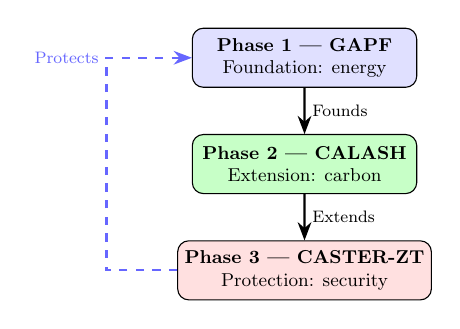
\begin{tikzpicture}[scale=0.75, every node/.style={scale=0.75},
      blk/.style={draw, rounded corners=4pt, minimum width=3.8cm, minimum height=1cm, align=center, font=\small}]
    \node[blk, fill=blue!12] (a1) at (0,0) {\textbf{Phase 1 --- GAPF}\\Foundation: energy};
    \node[blk, fill=green!22] (a2) at (0,-1.8) {\textbf{Phase 2 --- CALASH}\\Extension: carbon};
    \node[blk, fill=red!12] (a3) at (0,-3.6) {\textbf{Phase 3 --- CASTER-ZT}\\Protection: security};
    \draw[-{Stealth},thick] (a1) -- node[right,font=\footnotesize] {Founds} (a2);
    \draw[-{Stealth},thick] (a2) -- node[right,font=\footnotesize] {Extends} (a3);
    \draw[-{Stealth},thick,dashed,blue!60] (a3.west) -- ++(-1.2,0) |- (a1.west) node[midway, left, font=\footnotesize, align=center] {Protects};
  \end{tikzpicture}
\end{column}
\end{columns}
\end{frame}

% ============================================================
\begin{frame}{Common Experimental Protocol}
\begin{columns}[T]
\begin{column}{0.48\textwidth}
  \begin{block}{Simulation Environment}
    \begin{itemize}\small
      \item Python + PyTorch, PyMARL2
      \item Heinzelman first-order energy model
      \item Real-world data: Intel Lab, UK Carbon Intensity API, USGS ShakeMap
      \item Seismic model calibrated on Turkey--Syria 2023
    \end{itemize}
  \end{block}
\end{column}
\begin{column}{0.48\textwidth}
  \begin{block}{Statistical Rigor}
    \begin{itemize}\small
      \item Article 1: 21,000 runs, 7 scenarios
      \item Article 2: 390 runs, 30 Monte Carlo seeds
      \item Article 3: 2,420 runs
      \item Total: $>$ 23,800 runs
      \item Statistical tests: 95\% CI, Wilcoxon, bootstrap
    \end{itemize}
  \end{block}
\end{column}
\end{columns}
\end{frame}

% ============================================================
\section{Article 1 --- GAPF}
% ============================================================

\begin{frame}{GAPF: Graph-Attentive Policy Fusion}
{\small\color{polyblue} \textbf{G.\,P.\ Djimefo Kapen}, \textbf{R.\ Al Mallah}, \textbf{S.\ Pierre} --- \textit{IEEE Trans.\ Green Comm.\ \& Netw.}}
\vspace{2pt}
\begin{block}{Key Idea}
  Fuse complementary frozen MARL expert policies (QMIX \& QTRAN) via a lightweight GNN encoder, instead of training a heavier monolithic network.
\end{block}

\vspace{4pt}
\centering
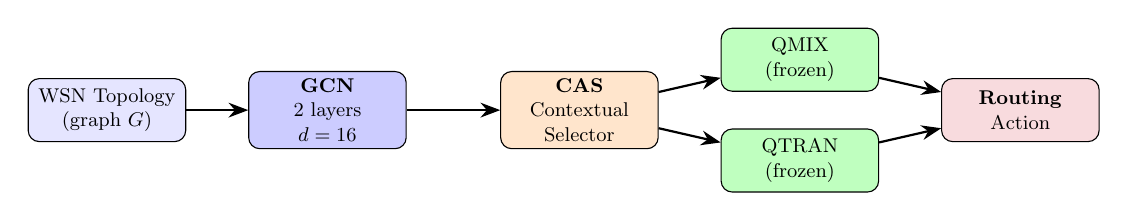
\begin{tikzpicture}[scale=0.8, every node/.style={scale=0.8},
    box/.style={draw, rounded corners, minimum width=2.5cm, minimum height=1cm, align=center, font=\small},
    arr/.style={-{Stealth[length=2.5mm]}, thick}]
  % Inputs
  \node[box, fill=blue!10] (topo) at (-4,0) {WSN Topology\\(graph $G$)};
  % GCN
  \node[box, fill=blue!20] (gcn) at (-0.5,0) {\textbf{GCN}\\2 layers\\$d=16$};
  % CAS
  \node[box, fill=orange!20] (cas) at (3.5,0) {\textbf{CAS}\\Contextual\\Selector};
  % Experts
  \node[box, fill=green!25] (qmix) at (7,0.8) {QMIX\\(frozen)};
  \node[box, fill=green!25] (qtran) at (7,-0.8) {QTRAN\\(frozen)};
  % Output
  \node[box, fill=polyred!15] (act) at (10.5,0) {\textbf{Routing}\\Action};

  \draw[arr] (topo) -- (gcn);
  \draw[arr] (gcn) -- (cas);
  \draw[arr] (cas) -- (qmix);
  \draw[arr] (cas) -- (qtran);
  \draw[arr] (qmix) -- (act);
  \draw[arr] (qtran) -- (act);
\end{tikzpicture}

\vspace{6pt}
\small
\begin{columns}[T]
\begin{column}{0.48\textwidth}
  \begin{itemize}
    \item GCN: encodes topology into a compact embedding
    \item CAS: contextual selection of the optimal expert
  \end{itemize}
\end{column}
\begin{column}{0.48\textwidth}
  \begin{itemize}
    \item Monotonic Q$\cdot$K Attention Network for multi-objective reward scalarization
    \item Tri-component: REINFORCE (GCN+CAS) + ES (Q$\cdot$K attention) outer; MARL inner
  \end{itemize}
\end{column}
\end{columns}
\end{frame}

% ============================================================
\begin{frame}[t]{GAPF: Why Fusion Works}
\begin{columns}[T]
\begin{column}{0.47\textwidth}
  \begin{block}{QMIX / QTRAN Complementarity}
    \begin{itemize}\small\setlength{\itemsep}{1pt}
      \item \textbf{QMIX}: $\partial Q_\text{tot}/\partial Q_i \geq 0$ $\Rightarrow$ tight coordination
      \item \textbf{QTRAN}: affine transforms $\Rightarrow$ non-monotonic interactions
      \item CAS selects expert by topological context
    \end{itemize}
  \end{block}
\end{column}
\begin{column}{0.47\textwidth}
  \begin{block}{Monotonic Q$\cdot$K Attention}
    \begin{itemize}\small\setlength{\itemsep}{1pt}
      \item Multi-objective scalarization (energy, PDR, latency)
      \item Non-negative weights $\Rightarrow$ \textbf{Pareto monotonicity}
      \item Dominance $\Rightarrow$ higher scalar score
      \item Eliminates classical scalarization artifacts
    \end{itemize}
  \end{block}
\end{column}
\end{columns}
\vspace{2pt}
\begin{exampleblock}{``Expert Portfolio'' Paradigm}
  \centering\small
  Established in combinatorial optimization --- applied 1\textsuperscript{st} time to MARL routing in WSNs.
\end{exampleblock}
\end{frame}

% ============================================================
\begin{frame}[shrink=8]{GAPF: Key Results}
\centering
\renewcommand{\arraystretch}{1.2}
\begin{tabular}{lccr}
  \toprule
  \textbf{Metric} & \textbf{Baseline (QMIX)} & \textbf{GAPF} & \textbf{Gain} \\
  \midrule
  PDR (delivery ratio) & 46--67\% & $\geq$ \textbf{98\%} & +43--111\% $\uparrow$ \\
  Energy per packet & $1.0\times$ & $0.29$--$0.50\times$ & \textbf{2--3.5$\times$ $\downarrow$} \\
  Trainable parameters & $\sim$39K/agent & \textbf{1,473} & 26$\times$ $\downarrow$ \\
  Training memory & 3.2--13.8\,GB & \textbf{951\,MB} & 3.4--14.5$\times$ $\downarrow$ \\
  Model size & --- & \textbf{5.8\,KB} & Cortex-M4 OK \\
  \bottomrule
\end{tabular}

\vspace{10pt}
\begin{columns}
\begin{column}{0.48\textwidth}
  \begin{exampleblock}{\faCheck\; Contributions}
    \begin{itemize}\small
      \item 1\textsuperscript{st} MARL policy fusion framework via GNN for WSNs
      \item 26$\times$ fewer parameters than an RNN agent
      \item Deployable on microcontroller without compression
    \end{itemize}
  \end{exampleblock}
\end{column}
\begin{column}{0.48\textwidth}
  \begin{block}{Validated on}
    \begin{itemize}\small
      \item 7 scenarios (20--100 sensors)
      \item 21,000 test episodes
      \item Compared to QMIX, QTRAN, QPSOFL
    \end{itemize}
  \end{block}
\end{column}
\end{columns}
\end{frame}

% ============================================================
\section{Article 2 --- CALASH}
% ============================================================

\begin{frame}[t]{CALASH: Carbon-Aware Lifecycle-Autonomous Self-Healing}
{\small\color{polyblue} \textbf{G.\,P.\ Djimefo Kapen}, \textbf{R.\ Al Mallah}, \textbf{S.\ Pierre} --- \textit{IEEE Trans.\ Green Comm.\ \& Netw.}}
\vspace{2pt}
\begin{block}{Fundamental Insight}
  \small Embodied carbon dominates operational by $10^6\!:\!1$ in WSNs. Real lever: \textbf{maximize useful delivered packets} to amortize embodied carbon.
\end{block}
\vspace{1pt}
\centering
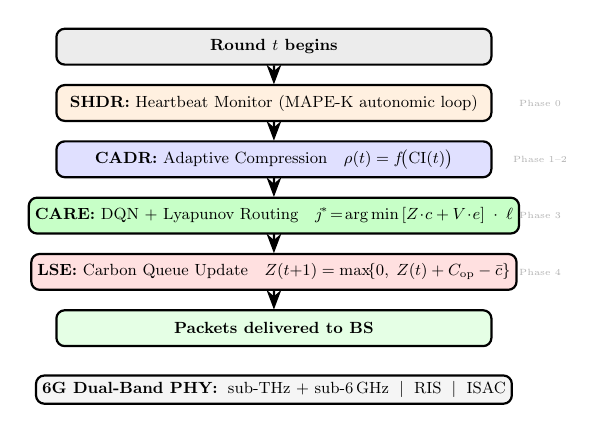
\begin{tikzpicture}[scale=0.65, every node/.style={scale=0.65},
    phase/.style={draw, thick, rounded corners=3pt,
      minimum width=8.5cm, minimum height=0.7cm,
      align=center, font=\small},
    arr/.style={-{Stealth[length=2.5mm]}, thick},
    phlbl/.style={font=\tiny, text=gray!60}]
  % --- Per-round vertical flow (faithful to article figure) ---
  \node[phase, fill=gray!15] (round) at (0,0)
    {\textbf{Round $t$ begins}};
  \node[phase, fill=orange!12] (shdr) at (0,-1.1)
    {\textbf{SHDR:} Heartbeat Monitor (MAPE-K autonomic loop)};
  \node[phase, fill=blue!12] (cadr) at (0,-2.2)
    {\textbf{CADR:} Adaptive Compression\quad
     $\rho(t) = f\!\big(\text{CI}(t)\big)$};
  \node[phase, fill=green!22] (care) at (0,-3.3)
    {\textbf{CARE:} DQN + Lyapunov Routing\quad
     $j^{\!*} \!=\! \arg\min\,[Z\!\cdot\!c + V\!\cdot\!e]\;\cdot\;\ell$};
  \node[phase, fill=red!12] (lse) at (0,-4.4)
    {\textbf{LSE:} Carbon Queue Update\quad
     $Z(t{+}1) = \max\!\{0,\; Z(t) + C_{\text{op}} - \bar{c}\}$};
  \node[phase, fill=green!10] (out) at (0,-5.5)
    {\textbf{Packets delivered to BS}};
  % --- Arrows ---
  \draw[arr] (round) -- (shdr);
  \draw[arr] (shdr)  -- (cadr);
  \draw[arr] (cadr)  -- (care);
  \draw[arr] (care)  -- (lse);
  \draw[arr] (lse)   -- (out);
  % --- Phase labels ---
  \node[phlbl] at (5.2,-1.1) {Phase 0};
  \node[phlbl] at (5.2,-2.2) {Phase 1--2};
  \node[phlbl] at (5.2,-3.3) {Phase 3};
  \node[phlbl] at (5.2,-4.4) {Phase 4};
  % --- 6G PHY foundation layer ---
  \node[draw, thick, fill=gray!8, rounded corners=3pt,
        minimum width=8.5cm, minimum height=0.55cm,
        align=center, font=\small]
    at (0,-6.7)
    {\textbf{6G Dual-Band PHY:}\; sub-THz + sub-6\,GHz
     \;\textbar\; RIS \;\textbar\; ISAC};
\end{tikzpicture}
\end{frame}

% ============================================================
\begin{frame}[t]{CALASH: The Four Pillars in Detail}
\begin{columns}[T]
\begin{column}{0.48\textwidth}
  \begin{block}{\faDatabase\; CADR --- Data Reduction}
    \begin{itemize}\small\setlength{\itemsep}{1pt}
      \item Sensing ratio modulated by grid carbon intensity
      \item ``Dirty'' electricity: compress more
      \item ``Clean'' electricity: compress less
    \end{itemize}
  \end{block}
  \vspace{1pt}
  \begin{block}{\faRecycle\; SHDR --- Self-Healing}
    \begin{itemize}\small\setlength{\itemsep}{1pt}
      \item Autonomic MAPE-K loop
      \item Detects dead nodes post-disaster
      \item Rebuilds topology automatically
    \end{itemize}
  \end{block}
\end{column}
\begin{column}{0.48\textwidth}
  \begin{block}{\faRoute\; CARE --- Carbon-Aware Routing}
    \begin{itemize}\small\setlength{\itemsep}{1pt}
      \item Hybrid Lyapunov + DQN router
      \item Virtual carbon queue $\Rightarrow$ drift-plus-penalty
      \item \textbf{CDL Pareto bound}: provable convergence
    \end{itemize}
  \end{block}
  \vspace{1pt}
  \begin{block}{\faBalanceScale\; LSE --- Lifecycle Engine}
    \begin{itemize}\small\setlength{\itemsep}{1pt}
      \item ISO 14040 compliant
      \item Manufacturing + operation + end-of-life
      \item LCI: gCO$_2$eq / useful packet
    \end{itemize}
  \end{block}
\end{column}
\end{columns}
\end{frame}

% ============================================================
\begin{frame}[shrink=8]{CALASH: Key Results}
\centering
\renewcommand{\arraystretch}{1.2}
\begin{tabular}{lccr}
  \toprule
  \textbf{Metric} & \textbf{Baseline (LEACH)} & \textbf{CALASH} & \textbf{Gain} \\
  \midrule
  Network lifetime & 931 rounds & \textbf{1,486 rounds} & +60\% \\
  PDR & --- & \textbf{82.9\%} & --- \\
  LCI (gCO$_2$eq/pkt) & 13.42 & \textbf{8.99} & $-$33\% \\
  Physical layer & classical & \textbf{6G dual-band} & sub-THz + RIS \\
  \bottomrule
\end{tabular}

\vspace{10pt}
\begin{columns}
\begin{column}{0.48\textwidth}
  \begin{exampleblock}{\faCheck\; Contributions}
    \begin{itemize}\small
      \item 1\textsuperscript{st} LCI metric for WSNs (ISO 14040)
      \item 1\textsuperscript{st} 4-pillar protocol with Lyapunov guarantees
      \item Insight: reducing transmitted volume $>$ reducing energy/packet
    \end{itemize}
  \end{exampleblock}
\end{column}
\begin{column}{0.48\textwidth}
  \begin{block}{Validated on}
    \begin{itemize}\small
      \item 390 runs, 30 Monte Carlo seeds
      \item Seismic model calibrated (Turkey 2023)
      \item UK Carbon Intensity API
      \item Compared to LEACH, HEED, EERP
    \end{itemize}
  \end{block}
\end{column}
\end{columns}
\end{frame}

% ============================================================
\section{Article 3 --- CASTER-ZT}
% ============================================================

\begin{frame}[shrink=5]{CASTER-ZT: Zero-Trust Shielded Decision Control}
{\small\color{polyblue} \textbf{G.\,P.\ Djimefo Kapen}, \textbf{R.\ Al Mallah}, \textbf{S.\ Pierre} --- \textit{IEEE Trans.\ Mobile Computing}}
\vspace{1pt}
\begin{block}{Observation}
  AI in the control loop creates a \textbf{new attack surface}. Existing mechanisms (CPO, binary shielding) only offer \emph{allow} or \emph{block} --- unsuitable for critical missions.
\end{block}

\vspace{1pt}
\centering
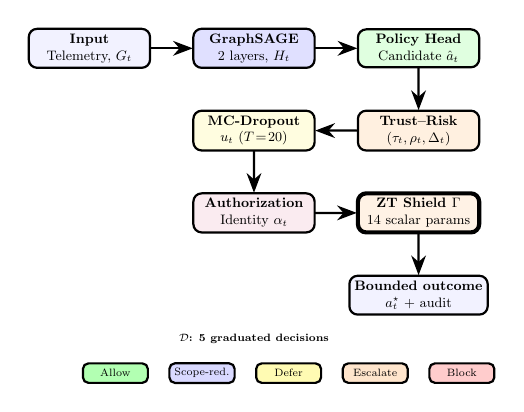
\begin{tikzpicture}[scale=0.55, every node/.style={scale=0.55},
    blk/.style={draw, thick, rounded corners=3pt,
      minimum width=2.8cm, minimum height=0.85cm,
      align=center, font=\small},
    shd/.style={blk, fill=orange!10, line width=1.5pt},
    dec/.style={draw, thick, rounded corners=2pt,
      minimum width=1.5cm, minimum height=0.45cm,
      align=center, font=\scriptsize},
    arr/.style={-{Stealth[length=2.5mm]}, thick}]
  % === Row 1: Input → Encoder → Policy Head ===
  \node[blk, fill=blue!5]  (inp) at (0,0)     {\textbf{Input}\\Telemetry, $G_t$};
  \node[blk, fill=blue!12] (enc) at (3.8,0)   {\textbf{GraphSAGE}\\2 layers, $H_t$};
  \node[blk, fill=green!12](pol) at (7.6,0)   {\textbf{Policy Head}\\Candidate $\hat{a}_t$};
  % === Row 2: Trust-Risk ← Uncertainty ===
  \node[blk, fill=orange!12](tr) at (7.6,-1.9)  {\textbf{Trust--Risk}\\$(\tau_t,\rho_t,\Delta_t)$};
  \node[blk, fill=yellow!12](uc) at (3.8,-1.9)  {\textbf{MC-Dropout}\\$u_t$ ($T\!=\!20$)};
  % === Row 3: Authorization → Shield ===
  \node[blk, fill=purple!8] (auth) at (3.8,-3.8) {\textbf{Authorization}\\Identity $\alpha_t$};
  \node[shd]                (sh)   at (7.6,-3.8) {\textbf{ZT Shield $\Gamma$}\\14 scalar params};
  % === Bounded output ===
  \node[blk, fill=blue!5]   (out)  at (7.6,-5.7) {\textbf{Bounded outcome}\\$a_t^\star$ + audit};
  % === Arrows (faithful zigzag dataflow) ===
  \draw[arr] (inp) -- (enc);
  \draw[arr] (enc) -- (pol);
  \draw[arr] (pol) -- (tr);
  \draw[arr] (tr)  -- (uc);
  \draw[arr] (uc)  -- (auth);
  \draw[arr] (auth) -- (sh);
  \draw[arr] (sh)  -- (out);
  % === 5 graduated decisions ===
  \node[font=\scriptsize\bfseries] at (3.8,-6.7) {$\mathcal{D}$: 5 graduated decisions};
  \node[dec, fill=green!30]  at (0.6,-7.5)   {Allow};
  \node[dec, fill=blue!15]   at (2.6,-7.5)   {Scope-red.};
  \node[dec, fill=yellow!30] at (4.6,-7.5)   {Defer};
  \node[dec, fill=orange!20] at (6.6,-7.5)   {Escalate};
  \node[dec, fill=red!20]    at (8.6,-7.5)   {Block};
\end{tikzpicture}

\vspace{3pt}
\small
\begin{columns}[T]
\begin{column}{0.48\textwidth}
  \begin{itemize}
    \item NIST SP 800-207 compliant (zero-trust)
    \item Every actuation verified in real time
  \end{itemize}
\end{column}
\begin{column}{0.48\textwidth}
  \begin{itemize}
    \item 10 formal propositions proven
    \item Shield is \textbf{explainable} and \textbf{auditable}
  \end{itemize}
\end{column}
\end{columns}
\end{frame}

% ============================================================
\begin{frame}[t]{CASTER-ZT: Formal Guarantees and Results}
\begin{columns}[T]
\begin{column}{0.47\textwidth}
  \begin{block}{10 Formal Propositions}
    \begin{itemize}\footnotesize\setlength{\itemsep}{1pt}
      \item Monotone conservatism
      \item Unauthorized-actuation exclusion
      \item Conformal coverage
      \item Graceful degradation
      \item Shield correctness \& completeness
    \end{itemize}
  \end{block}
  \vspace{1pt}
  \begin{alertblock}{Deterministic Shield}
    \footnotesize \textbf{14 scalar params}, non-learnable --- last defense if neural parts compromised.
  \end{alertblock}
\end{column}
\begin{column}{0.47\textwidth}
  \centering\footnotesize
  \renewcommand{\arraystretch}{1.05}
  \begin{tabular}{lcr}
    \toprule
    \textbf{Metric} & \textbf{CASTER-ZT} & \textbf{vs.\ baseline} \\
    \midrule
    Rogue detection & 74--98\% & +14--28 pts \\
    False positives & \textbf{0\%} & Full elim. \\
    $\omega_\text{rec}$ & 0.733 & 3.7--5.2$\times$ $\uparrow$ \\
    Latency/decision & \textbf{3.07\,ms} & 4.9$\times$ $\downarrow$ \\
    O-RAN budget & $\leq$ 10\,ms & \faCheck \\
    \bottomrule
  \end{tabular}
  \vspace{1pt}
  \begin{block}{Validated on}
    \footnotesize 2,420 runs, 100 hex.\ cells. Compared to CPO, binary shield.
  \end{block}
\end{column}
\end{columns}
\end{frame}

% ============================================================
\section{Discussion and Cross-Analysis}
% ============================================================

\begin{frame}[t]{Protocol Stack Synergies}
\centering
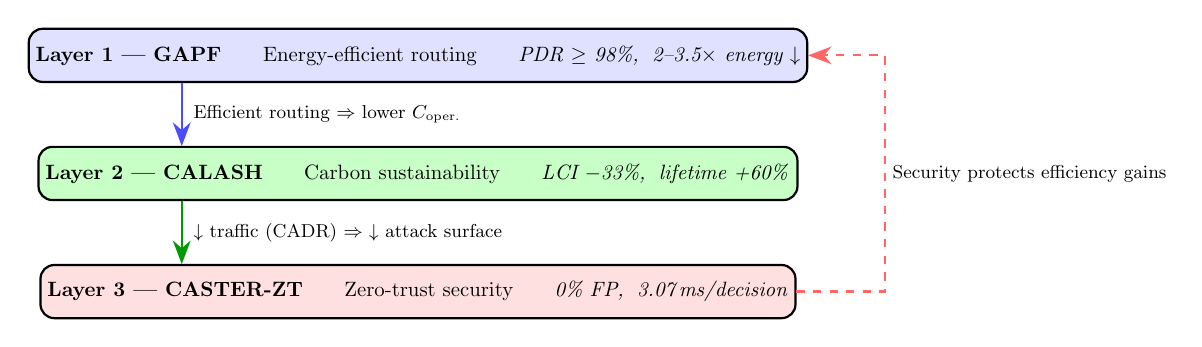
\begin{tikzpicture}[scale=0.75, every node/.style={scale=0.75},
    layer/.style={draw, thick, rounded corners=5pt, minimum width=12.5cm, minimum height=0.9cm, align=center, font=\normalsize}]
  \node[layer, fill=blue!12]  (l1) at (0,0)
    {\textbf{Layer~1 --- GAPF}\qquad Energy-efficient routing\qquad
     \textit{PDR~$\geq$~98\%,\; 2--3.5$\times$ energy~$\downarrow$}};
  \node[layer, fill=green!22] (l2) at (0,-2)
    {\textbf{Layer~2 --- CALASH}\qquad Carbon sustainability\qquad
     \textit{LCI~$-$33\%,\; lifetime~+60\%}};
  \node[layer, fill=red!12]   (l3) at (0,-4)
    {\textbf{Layer~3 --- CASTER-ZT}\qquad Zero-trust security\qquad
     \textit{0\%~FP,\; 3.07\,ms/decision}};

  % --- Down arrows anchored to box borders ---
  \draw[-{Stealth[length=3mm]}, thick, blue!70]
    ([xshift=-4cm]l1.south) -- ([xshift=-4cm]l2.north)
    node[midway, right, font=\small, text=black, xshift=2pt]
      {Efficient routing $\Rightarrow$ lower $C_{\text{oper.}}$};
  \draw[-{Stealth[length=3mm]}, thick, green!60!black]
    ([xshift=-4cm]l2.south) -- ([xshift=-4cm]l3.north)
    node[midway, right, font=\small, text=black, xshift=2pt]
      {$\downarrow$ traffic (CADR) $\Rightarrow$ $\downarrow$ attack surface};
  % --- Feedback arrow: L3 right → up → L1 right ---
  \draw[-{Stealth[length=3mm]}, thick, dashed, red!60]
    (l3.east) -- ++(1.5,0) |- (l1.east)
    node[pos=0.25, right, font=\small, text=black]
      {Security protects efficiency gains};
\end{tikzpicture}

\vspace{1pt}
\begin{columns}[T]
\begin{column}{0.48\textwidth}
  \begin{exampleblock}{Mutual Reinforcement}
    \small The three layers reinforce each other: efficiency $\to$ sustainability $\to$ security. No trade-off.
  \end{exampleblock}
\end{column}
\begin{column}{0.48\textwidth}
  \begin{block}{Total Cost}
    \small $\sim$27K params $\approx$ 1 RNN agent, $\sim$103\,KB (FP32) $\Rightarrow$ Cortex-M7 OK.
    Full stack $<$ one QMIX agent budget.
  \end{block}
\end{column}
\end{columns}
\end{frame}

% ============================================================
\begin{frame}{Overall Quantitative Summary}
\centering
\small
\renewcommand{\arraystretch}{1.15}
\begin{tabular}{@{}llccr@{}}
  \toprule
  \textbf{Metric} & \textbf{Best baseline} & \textbf{Baseline val.} & \textbf{Our result} & \textbf{Gain} \\
  \midrule
  PDR & QMIX & 46--67\% & $\geq$ \textbf{98\%} & +43--111\% $\uparrow$ \\
  Energy / packet & QMIX & $1.0\times$ & $0.29$--$0.50\times$ & 2--3.5$\times$ $\downarrow$ \\
  Parameters & RNN agent & $\sim$39K & \textbf{1,473} & 26$\times$ $\downarrow$ \\
  Training memory & QMIX & 3.2--13.8\,GB & \textbf{951\,MB} & 3.4--14.5$\times$ $\downarrow$ \\
  Network lifetime & LEACH & 931 rounds & \textbf{1,486 rounds} & +60\% \\
  LCI (CO$_2$/pkt) & LEACH & 13.42 & \textbf{8.99} & $-$33\% \\
  Rogue det.\ (0\% FP) & Best 0-FP & 0\% & \textbf{74--98\%} & +74--98 pts \\
  False positives & Shield-Binary & 48.8\% & \textbf{0\%} & Full elim. \\
  Latency / decision & O-RAN budget & 10\,ms & \textbf{3.07\,ms} & 3.3$\times$ $\downarrow$ \\
  Criteria covered (/12) & Best existing & 1 & \textbf{12} & 12$\times$ $\uparrow$ \\
  \midrule
  \multicolumn{4}{l}{\textbf{Total test runs}} & $>$ \textbf{23,800} \\
  \bottomrule
\end{tabular}
\end{frame}

% ============================================================
\begin{frame}[shrink=5]{TinyML Deployability}
\centering
\renewcommand{\arraystretch}{1.2}
\begin{tabular}{lcccl}
  \toprule
  \textbf{Framework} & \textbf{Params} & \textbf{Memory} & \textbf{Target} & \textbf{Compression} \\
  \midrule
  GAPF & 1,473 & 5.8\,KB & Cortex-M4 & None needed \\
  CALASH & $\sim$5K & 19.5\,KB & Cortex-M4 & INT8 ($\to$4.9\,KB) \\
  CASTER-ZT & $\sim$20K & 78\,KB & Cortex-M7 & Distill.+INT8 ($\to$20\,KB) \\
  \midrule
  \textbf{Full stack} & $\sim$\textbf{27K} & \textbf{103\,KB} & \textbf{Cortex-M7} & Mixed quant. \\
  \bottomrule
\end{tabular}

\vspace{10pt}
\begin{columns}[T]
\begin{column}{0.48\textwidth}
  \begin{exampleblock}{Comparison}
    \small MCUNet deploys $\sim$1M parameters on Cortex-M7.\\
    Our stack: $\sim$27K $\Rightarrow$ \textbf{38$\times$ lighter}.
  \end{exampleblock}
\end{column}
\begin{column}{0.48\textwidth}
  \begin{block}{Implication}
    \small Deployable on microcontrollers costing a few dollars $\Rightarrow$ accessible to developing countries (where 95\% of deaths occur).
  \end{block}
\end{column}
\end{columns}
\end{frame}

% ============================================================
\section{Contributions and Impact}
% ============================================================

\begin{frame}{Six Original Scientific Contributions}
\begin{enumerate}\small
  \item \textbf{C1}: First \textbf{MARL policy fusion framework via GNN} for WSN routing\\
        {\footnotesize GNN+CAS paradigm transferable to any multi-agent system}

  \item \textbf{C2}: \textbf{Monotonic Q$\cdot$K Attention Network} for multi-objective scalarization\\
        {\footnotesize Pareto monotonicity formally guaranteed --- absent from existing methods}

  \item \textbf{C3}: First \textbf{Lifecycle Carbon Intensity (LCI)} metric for WSNs\\
        {\footnotesize ISO 14040 compliant --- adoptable for any IoT protocol}

  \item \textbf{C4}: First \textbf{4-pillar protocol with Lyapunov guarantees} for carbon budget\\
        {\footnotesize Provable convergence to near-optimal PDR AND bounded carbon budget}

  \item \textbf{C5}: First \textbf{zero-trust decision control} framework for AI-native networks\\
        {\footnotesize 5 graduated decisions + 10 formal propositions + explainable shield}

  \item \textbf{C6}: Demonstration of \textbf{complementarity} between efficiency--sustainability--security\\
        {\footnotesize Integrated protocol stack: all 3 objectives reinforce each other}
\end{enumerate}
\end{frame}

% ============================================================
\begin{frame}[t]{Impact and SDG Alignment}
\begin{columns}[T]
\begin{column}{0.47\textwidth}
  \begin{block}{\faBriefcase\; For Industry}
    \begin{itemize}\footnotesize\setlength{\itemsep}{1pt}
      \item GAPF (5.8\,KB): no costly gateway
      \item +60\% lifetime $\Rightarrow$ $\downarrow$ maintenance
      \item LCI: sustainability reporting (CSRD/SEC)
      \item Auditable shield: IEC 62443
    \end{itemize}
  \end{block}
  \vspace{1pt}
  \begin{block}{\faUniversity\; For Governments}
    \begin{itemize}\footnotesize\setlength{\itemsep}{1pt}
      \item LCI: standardized IoT indicator
      \item Sendai indicators C-2, C-6
      \item Open access, no proprietary lock-in
    \end{itemize}
  \end{block}
\end{column}
\begin{column}{0.47\textwidth}
  \footnotesize
  \renewcommand{\arraystretch}{1.0}
  \begin{tabular}{@{}cl@{}}
    \toprule
    \textbf{SDG} & \textbf{Contribution} \\
    \midrule
    \textbf{9} & Resilient infrastructure (1,473 params) \\
    \textbf{11} & Reduce losses (PDR $\geq$ 98\%) \\
    \textbf{12} & Sustainability (LCI ISO 14040) \\
    \textbf{13} & Climate resilience (CADR) \\
    \textbf{16} & Transparency (shield 0 FP) \\
    \bottomrule
  \end{tabular}
  \vspace{1pt}
  \begin{block}{\faUsers\; For Society}
    \begin{itemize}\footnotesize\setlength{\itemsep}{1pt}
      \item PDR $\geq$ 98\%: reliable alerts
      \item $-$33\% LCI: toward carbon neutrality
      \item SHDR: post-disaster coverage
    \end{itemize}
  \end{block}
\end{column}
\end{columns}
\end{frame}

% ============================================================
\section{Limitations and Future Work}
% ============================================================

\begin{frame}[t]{Acknowledged Limitations}
\begin{columns}[T]
\begin{column}{0.47\textwidth}
  \begin{alertblock}{Methodological}
    \begin{enumerate}\footnotesize\setlength{\itemsep}{2pt}
      \item \textbf{Simulation-based} --- real data but no hardware
      \item \textbf{Simplified disaster model} --- Gaussian, no cascades
      \item \textbf{Analytical 6G PHY} --- no 3D ray tracing
    \end{enumerate}
  \end{alertblock}
\end{column}
\begin{column}{0.47\textwidth}
  \begin{alertblock}{Technical}
    \begin{enumerate}\setcounter{enumi}{3}\footnotesize\setlength{\itemsep}{2pt}
      \item \textbf{Unvalidated integration} --- not tested as stack
      \item \textbf{Scalability $>$\,200 nodes} --- not characterized
      \item \textbf{Adaptive adversaries} --- static rogues only
      \item \textbf{No field validation} --- no user study
    \end{enumerate}
  \end{alertblock}
\end{column}
\end{columns}
\end{frame}

% ============================================================
\begin{frame}[t]{Future Research Directions}
\begin{columns}[T]
\begin{column}{0.31\textwidth}
  \begin{block}{\faCalendar\; Short (1--2\,yr)}
    \begin{itemize}\footnotesize\setlength{\itemsep}{1pt}
      \item Unified stack integration
      \item Hardware testbed (Zolertia, Coral, Jetson)
      \item Extended disaster models
    \end{itemize}
  \end{block}
\end{column}
\begin{column}{0.31\textwidth}
  \begin{block}{\faCalendar\; Medium (2--4\,yr)}
    \begin{itemize}\footnotesize\setlength{\itemsep}{1pt}
      \item Federated learning
      \item O-RAN digital twins
      \item Multi-disaster / multi-site
      \item Formal cert.\ (Coq/Isabelle)
    \end{itemize}
  \end{block}
\end{column}
\begin{column}{0.31\textwidth}
  \begin{block}{\faCalendar\; Long (4+\,yr)}
    \begin{itemize}\footnotesize\setlength{\itemsep}{1pt}
      \item Non-terrestrial (LEO, HAPS)
      \item LLMs as meta-controllers
      \item Standardization (ISO, 3GPP)
    \end{itemize}
  \end{block}
\end{column}
\end{columns}
\vspace{4pt}
{\centering\footnotesize\textbf{Transferability:} Precision agriculture~|~Smart cities~|~Connected health~|~Drone swarms\par}
\end{frame}

% ============================================================
\section{Conclusion}
% ============================================================

\begin{frame}[shrink=8]{Conclusion}
\begin{block}{Summary}
  This thesis proposed a \textbf{complete protocol stack} for intelligent routing in 6G-integrated disaster-monitoring WSNs, built around three complementary frameworks:
\end{block}

\vspace{4pt}
\begin{columns}[T]
\begin{column}{0.31\textwidth}
  \centering
  {\Large \faLightbulb}\par\vspace{4pt}
  \textbf{GAPF}\par
  {\small MARL fusion via GNN\par
  1,473 params, PDR $\geq$ 98\%\par
  Energy 2--3.5$\times$ $\downarrow$\par}
\end{column}
\begin{column}{0.31\textwidth}
  \centering
  {\Large \faLeaf}\par\vspace{4pt}
  \textbf{CALASH}\par
  {\small 4 pillars + 6G PHY\par
  LCI $-$33\%, lifetime +60\%\par
  CDL Pareto bound\par}
\end{column}
\begin{column}{0.31\textwidth}
  \centering
  {\Large \faLock}\par\vspace{4pt}
  \textbf{CASTER-ZT}\par
  {\small 5 graduated decisions\par
  0\% FP, 3.07\,ms\par
  10 formal propositions\par}
\end{column}
\end{columns}

\vspace{8pt}
\begin{exampleblock}{Key Message}
  \centering
  AI, designed with \textbf{parsimony} ($\sim$27K params), \textbf{environmental awareness} (LCI), and \textbf{systematic verification} (zero-trust), is a reliable tool for critical environments.
\end{exampleblock}
\end{frame}

% ============================================================
%  THANK YOU / QUESTIONS
% ============================================================
{
\setbeamertemplate{footline}{}
\begin{frame}[plain]
\vfill
\begin{center}
  
\includegraphics[height=1.2cm]{Polytechnique_Montreal_Logo.png}\hspace{2cm}%
  
\includegraphics[height=1.2cm]{Larim_logo.png}

  \vspace{0.6cm}
  {\Huge \textbf{Thank You!}}

  \vspace{0.5cm}
  {\LARGE Questions?}

  \vspace{0.8cm}
  {\large Georges Parfait \textsc{Djimefo Kapen}}\\[4pt]
  {\small Director: \textbf{Ranwa Al Mallah}}\\[2pt]
  {\small Co-director: \textbf{Samuel Pierre}}\\[6pt]
  {\small Department of Computer and Software Engineering}\\
  {\small Polytechnique Montr\'{e}al}

  \vspace{0.5cm}
  {\small\color{polyblue} \emph{AI-Driven Intelligent Routing and Secure Autonomous Recovery\\in 6G-Integrated Disaster-Monitoring Sensor Networks}}
\end{center}
\vfill
\end{frame}
}

% ============================================================
%  BACKUP SLIDES
% ============================================================
\appendix
\begin{frame}[plain]
  \centering
  {\Large \textbf{Backup Slides}}
\end{frame}

\begin{frame}[shrink=8]{Convergence and Theoretical Guarantees}
\begin{columns}[T]
\begin{column}{0.31\textwidth}
  \begin{block}{GAPF}
    \begin{itemize}\small
      \item QMIX: converges within the class of monotonic functions (IGM)
      \item QTRAN: larger space via affine factorization
      \item CAS: \emph{variance reducer} (Wolpert's stacking)
      \item Inference: $O(|E| \cdot d)$ for GCN
    \end{itemize}
  \end{block}
\end{column}
\begin{column}{0.31\textwidth}
  \begin{block}{CALASH}
    \begin{itemize}\small
      \item Lyapunov drift-plus-penalty optimization
      \item $O(1/V)$ convergence to optimum
      \item $V=100$: $-$33\% LCI + acceptable latency
      \item CDL bound: \emph{simultaneous} convergence PDR + carbon budget
    \end{itemize}
  \end{block}
\end{column}
\begin{column}{0.31\textwidth}
  \begin{block}{CASTER-ZT}
    \begin{itemize}\small
      \item 10 formal propositions
      \item Proved by logical construction
      \item Monotonicity, exclusion, coverage
      \item Shield is correct and complete
    \end{itemize}
  \end{block}
\end{column}
\end{columns}
\end{frame}

\begin{frame}[t]{Gap Analysis: Coverage of 12 Criteria}
\centering
\footnotesize
\renewcommand{\arraystretch}{0.95}
\begin{tabular}{@{}lcccc@{}}
  \toprule
  \textbf{Criterion} & \textbf{LEACH} & \textbf{QMIX} & \textbf{CPO} & \textbf{Our stack} \\
  \midrule
  Energy-efficient routing & \faCheck & \faCheck & & \faCheck \\
  Topology awareness (GNN) & & & & \faCheck \\
  MARL policy fusion & & & & \faCheck \\
  Pareto-monotonic scalarization & & & & \faCheck \\
  Lifecycle carbon metric & & & & \faCheck \\
  Carbon-aware data reduction & & & & \faCheck \\
  Carbon budget guarantees & & & & \faCheck \\
  Post-disaster self-healing & & & & \faCheck \\
  6G physical layer & & & & \faCheck \\
  Rogue policy detection & & & \faCheck & \faCheck \\
  Graduated decisions (5 levels) & & & & \faCheck \\
  Formal security guarantees & & & & \faCheck \\
  \midrule
  \textbf{Total (/12)} & \textbf{1} & \textbf{1} & \textbf{1} & \textbf{12} \\
  \bottomrule
\end{tabular}
\end{frame}

\begin{frame}{Dec-POMDP Complexity and Positioning}
\begin{block}{Theoretical Context}
  \begin{itemize}\small
    \item Optimal Dec-POMDP resolution: \textbf{NEXP-complete}
    \item CTDE (QMIX, QTRAN): structured approximation reducing $|\mathcal{A}|^n \to \sum_i |\mathcal{A}_i|$
    \item GAPF: adds expert selection as an additional level
    \item PDR $\geq$ 98\% is not guaranteed \emph{optimal} in the absolute sense, but constitutes a high-quality approximation
  \end{itemize}
\end{block}

\vspace{4pt}
\begin{block}{Positioning in the Value Decomposition Landscape}
  \begin{itemize}\small
    \item QMIX $\to$ WQMIX $\to$ QPLEX $\to$ FOP: increasingly heavy architectures
    \item GAPF: \textbf{orthogonal} path --- fusing lightweight experts via a topology-informed meta-controller
    \item ``Portfolio'' paradigm: well-established in combinatorial optimization, novel for MARL routing
  \end{itemize}
\end{block}
\end{frame}

\end{document}
